%!TeX root= ../thesis.tex
\section{UML}

The \ac{UML} is a standard language for modeling, building and documenting the design of a software system. It is often defined as the language in which the system's blueprint is written. In fact, various aspects of the system can be described by UML diagrams: use cases, interactions between different components, various logical and physical elements.
In this chapter, we will describe the logical system of the preference elicitation software developed to accompany the article in \cref{ch:minimax}.
In particular, we will illustrate the classes that constitute the various components of the system and the relationships between them.
A class describes the attributes and the properties of a group of objects. An object is an instance of a class.
Classes may inherit from other classes their actions and attributes. They can and implement abstract methods and add new functionality. Associations between classes represent these behaviors.

A class is represented as follows:

\begin{center}
	\begin{tikzpicture}
		\umlclass[y=-3]{Class}{
			+ d : double \\ - i : int \\ \# b : boolean
		}{ + equals(c : Class) : Boolean \\ + toString() : String \\ + hashCode() : Integer}
	\end{tikzpicture}
\end{center}

As we can see, the description of a class is divided into three sections, in the first there is its name, in the second its attributes and in the third its methods or behaviors. Attributes and methods can be either private $(-)$ to the class itself, protected $(\#)$ to the class and its children, or public $(+)$ to every other class.

In the example presented here there is a class named \textit{Class} with three attributes: a public attribute named $d$ of type \textit{double}, a private attribute named $i$ of type \textit{int} and a protected attribute named $b$ of type \textit{boolean}. Moreover, \textit{Class} has three methods:
\begin{itemize}[noitemsep]
	\item a method \textit{equals} which takes an element of the class \textit{Class} as input, compares it to the object on which this method is called and returns \textit{True} if they are the same objects, \textit{False} otherwise. The implementation of the method itself determine the meaning of similarity.
	\item a method \textit{toString} which does not take any input and returns the String corresponding to the current object. This value is often used for visualization purposes.
	\item a method \textit{hashCode} which does not take any input and produces an Integer value associated to the current object. This value is often used by the method \textit{equals} since same objects must return the same hash value. 
\end{itemize}

We described these three methods because they are basic methods that are automatically inherited by all classes. In fact, every class is an implicit child of a more general \textit{Object} class. If not specified these methods return the default mechanism that can lead to unexpected results. Although specified in our code, we decided to omit these methods from the uml diagrams as a matter of the clarity of the figure.

\subsection{Preference Representation}

\Cref{uml:preference} describes the basic elements of our elicitation software.
The two basic elements are represented by the \textit{Alternative} and \textit{Voter} objects. A \textit{Preference} is a list of alternatives in which the order represents the preference order. Multiple alternatives can have the same rank but it is not possible to have the same alternative multiple times. Methods allow, for example, to know the alternative in a given rank or, conversely, to know the rank of a given alternative.
A \textit{StrictPreference} is an extension of the Preference object. This means that it inherits all of its behaviors and attributes but can redefine a given mechanism. In particular, StrictPreference does not allow two alternatives to have the same rank.
A \textit{VoterStrictPreference} links a Voter to her StrictPreference.
A \textit{PrefGraph} is a graph of preferences that can be added or modified. Specifically, each node represents an alternative, and an arc from a node $a$ to a node $b$ means that the alternative $a$ is preferred over the alternative $b$.
A \textit{VoterPartialPreference} links a Voter to her PrefGraph.

\begin{sidewaysfigure}
	\centering
	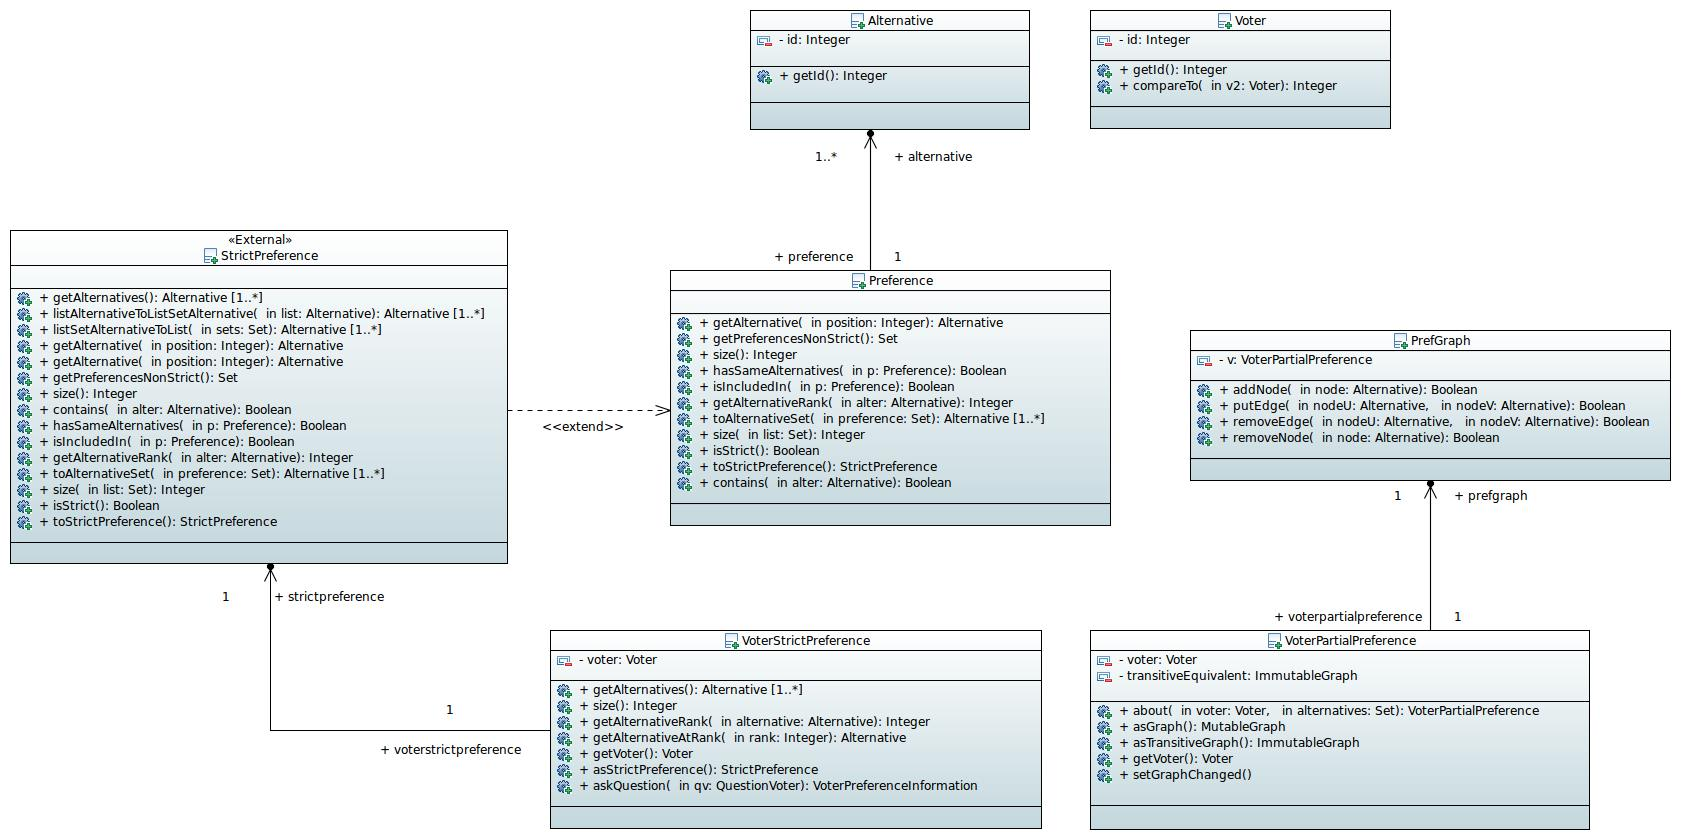
\includegraphics[width=\textwidth]{uml/basic.jpeg}
	\caption{UML class diagram of preferences representation.}
	\label{uml:preference}
\end{sidewaysfigure}

\subsection{Knowledge Representation}

\Cref{uml:knowledge} describes our approach to the representation of knowledge. We defined \textit{PreferenceKnowledge} as an interface, i.e. a completely abstract entity that define the structure that concrete objects must implement. An instance of PreferenceKnowledge must implements, among others, methods to return the alternatives, the voters, the profile and the constraints on the weights associated to rank positions.
A possible implementation is given by \textit{UpdateablePreferenceKnowledge} which keeps, as attributes, a partial profile and the constraints on weights and allows you to modify them. The \textit{ConstraintsOnWeights} are equations relating the difference between the weights of two consecutive pairs of ranks. It provides method to add constraints and to return an optimal set of weights that satisfies the constraints. Those weights are represented by \textit{PSRWeights} which is a list of rational numbers associated to the Positional Scoring Rule. Since in our framework we assume the convexity of weights the satisfaction of this condition is automatically checked when creating a new instance of this class.
Finally, in the diagram we can see an \textit{Oracle} class. This represents "true" knowledge, which exists but is unknown to us and which we try to elicit by asking questions. It contains the set of alternatives, the preferences of the chair\textemdash which are the weights of the scoring rule\textemdash and the preferences of the voters\textemdash which is the profile. During our elicitation procedure we ask questions to this entity.

\begin{sidewaysfigure}
	\centering
	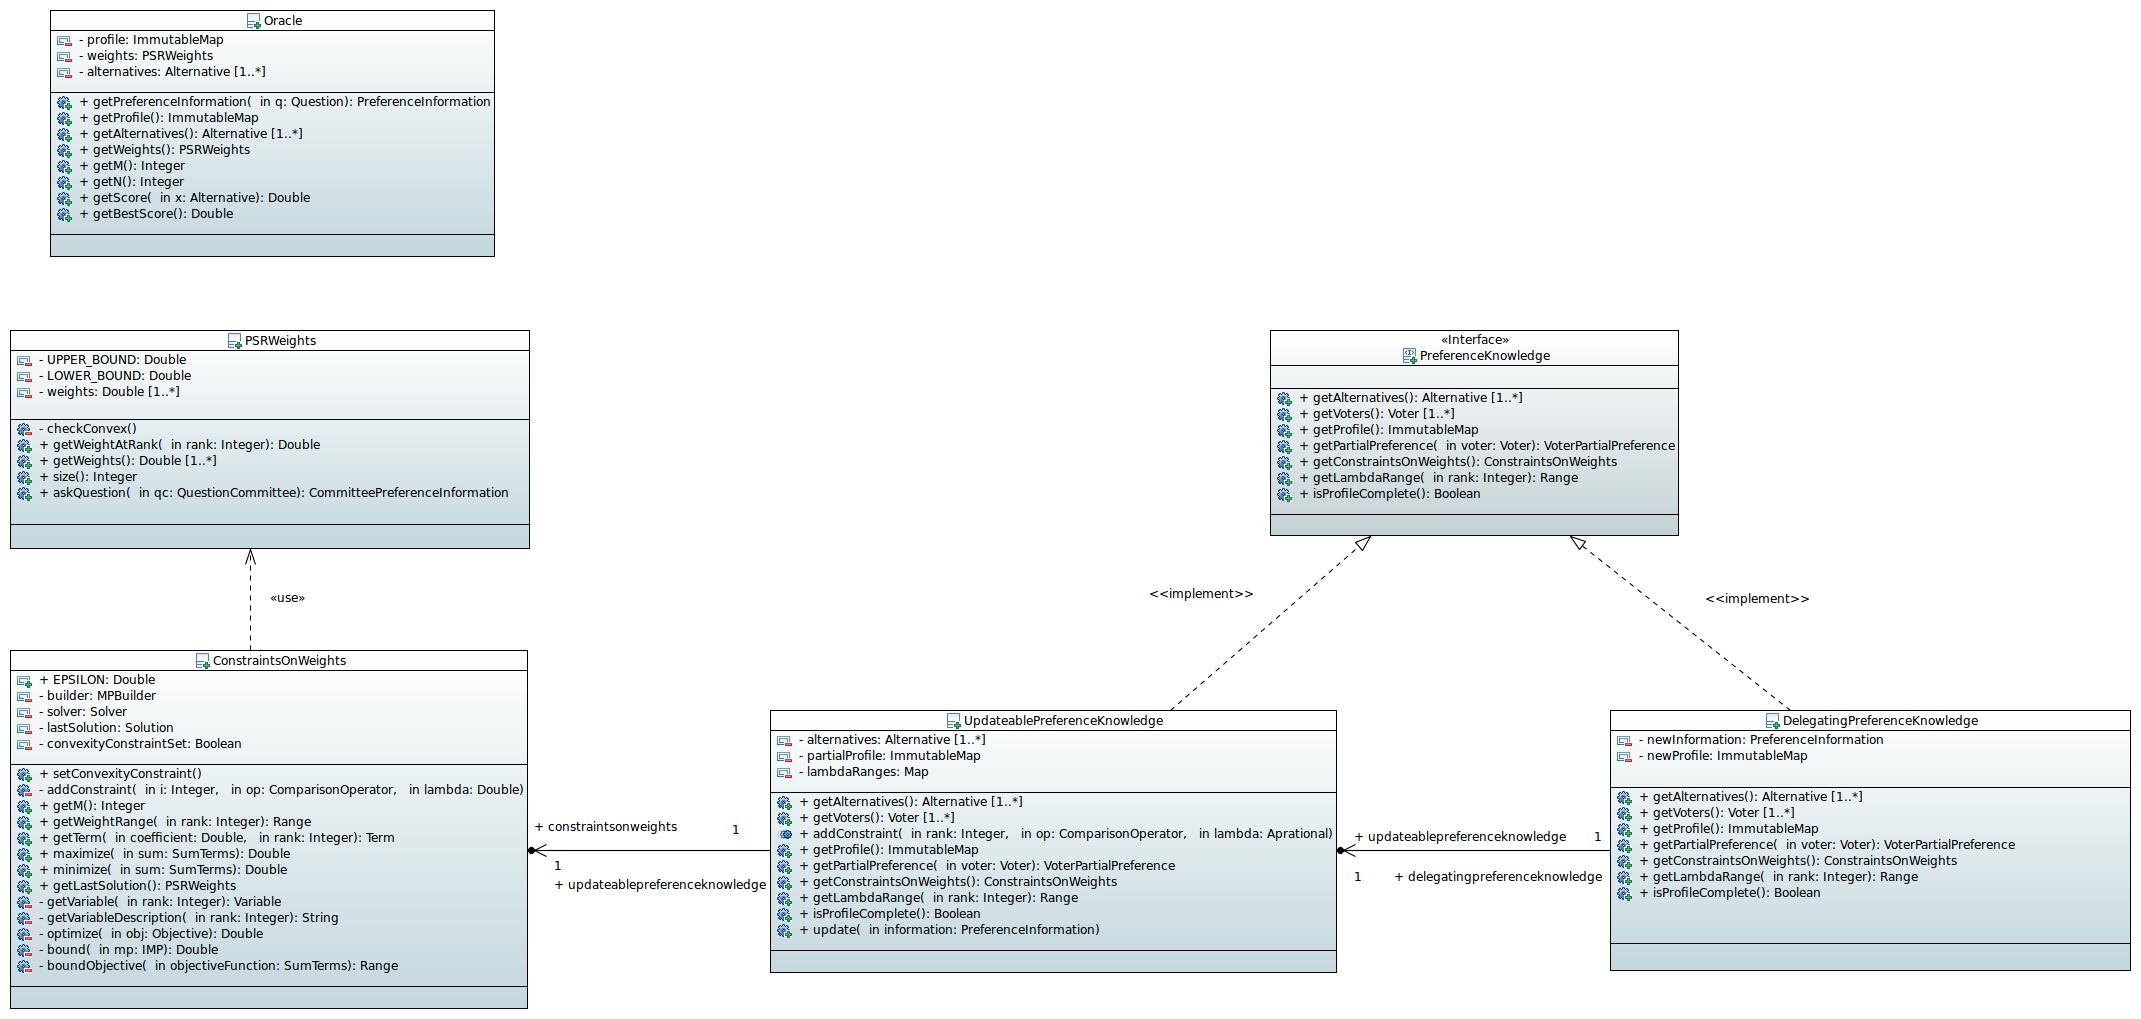
\includegraphics[width=\textwidth]{uml/knowledge.jpeg}
	\caption{UML class diagram of knowledge representation.}
	\label{uml:knowledge}
\end{sidewaysfigure}

\subsection{Questions Representation}

\Cref{uml:questions} shows the diagram related to the questions implementation. A \textit{Question} can be either a question to the chair, about their preferences on the voting rule, or a question to one of the voters, about their preferences over the alternatives. This is represented by the use of an enumeration \textit{QuestionType} that admits only two values: VOTER$\_$QUESTION and COMMITTEE$\_$QUE\\STION. %For Olivier: I know, I know, please accept it and don't blame me.
The method \textit{getType()} of \textit{Question} returns one of those two values.
A \textit{QuestionVoter} is a comparison query relating two alternatives $a$ and $b$, where \textit{getPositiveInformation()} returns the \textit{VoterPreferenceInformation} (see \Cref{uml:prefinfo}) associated to that specific voter and the alternative $a$ and $b$. Conversely, \textit{getNegativeInformation()} returns the information regarding the alternative $b$ and $a$. In other words, the first method returns the information when the answer to the question "$a\pref b ?$" is yes, thus $a$ is preferred to $b$, and the second method that when the answer is no, thus $b\pref a$.
A \textit{QuestionCommittee} try to improve the knowledge about the scoring rule by refining the multiplier $\lambda$ in the constraint $w_{r} - w_{r+1} \geq \lambda (w_{r+1} - w_{r+2})$ for some $r \in \{1,\ldots,m-2\}$. Given a $\lambda$ and a rank defined by an elicitation strategy, \textit{getPositiveInformation()} returns the response to the following question "$w_{r} - w_{r+1} \geq \lambda (w_{r+1} - w_{r+2})?$" is yes, while \textit{getNegativeInformation()} the information when the answer is no, thus $w_{r} - w_{r+1} \leq \lambda (w_{r+1} - w_{r+2})$.
Positive and negative information is used by the elicitation strategies for the choice of the next question to ask. In particular, the Pessimistic strategy consider, for each potential question, the information in case of positive and negative answer and pick the question that leads to minimal regret in the worst case. This is described in \Cref{uml:strategies}, in particular in the class diagram of \textit{MmrLottery}.

\vspace{2em}

\begin{figure}[h]
	\centering
	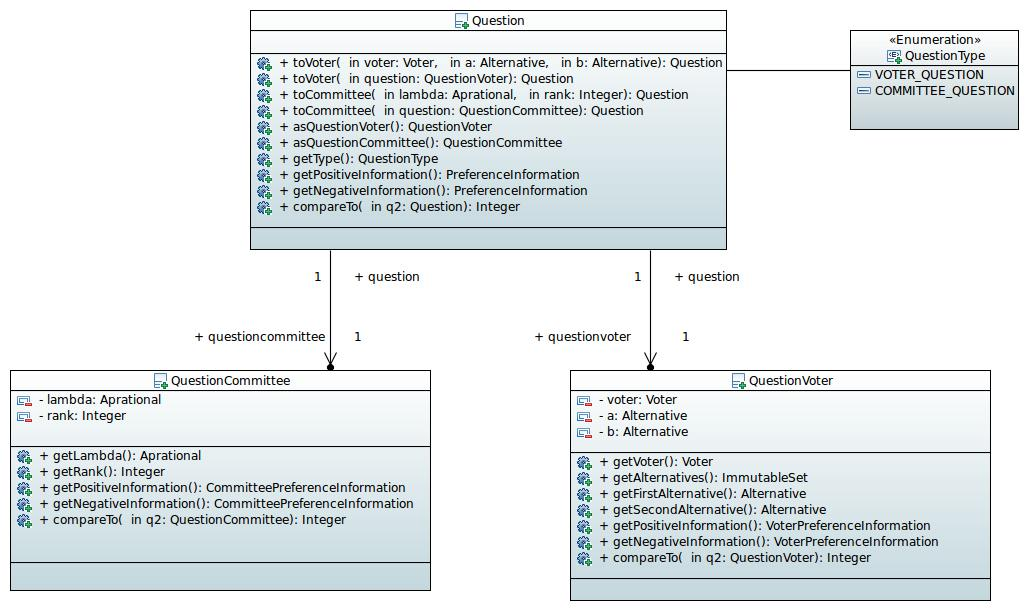
\includegraphics[width=\textwidth]{uml/questions.jpeg}
	\caption{UML class diagram of questions representation.}
	\label{uml:questions}
\end{figure}

\subsection{Preference Information}

\Cref{uml:prefinfo} illustrates the diagram related to the information about preferences acquired by asking questions. With a similar representation to the questions themselves, \textit{PreferenceInformation} can be of two types: \textit{CommitteePreferenceInformation} or \textit{VoterPreferenceInformation}. The type of the information depends on the type of the question asked.

\begin{figure}[h]
	\centering
	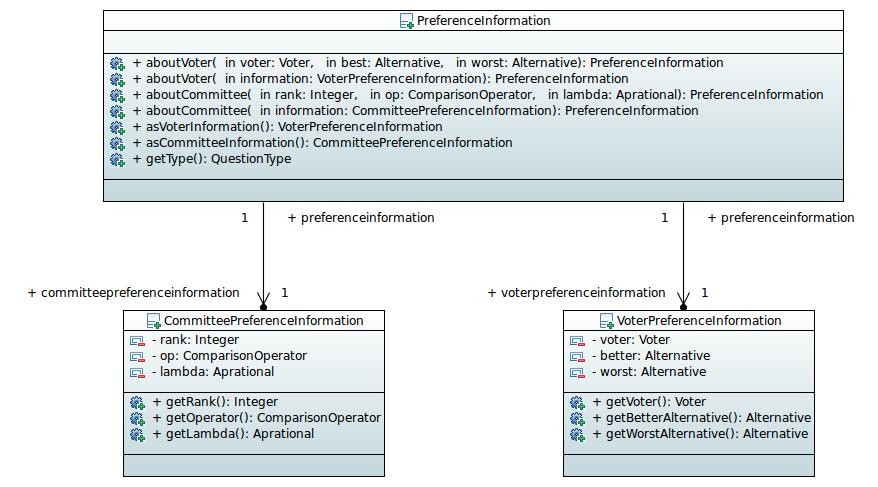
\includegraphics[width=\textwidth]{uml/prefinfo.jpeg}
	\caption{UML class diagram of elicited knowledge obtained by asking questions.}
	\label{uml:prefinfo}
\end{figure}

\subsection{Regret Computation}

\Cref{uml:regret} is the diagram representing the procedure described in \Cref{sec:mmr}. The \textit{PairwiseMaxRegret} is the building block of the regret computation. Given two alternatives, their ranks and the weights associated to ranks, it computes the regret of choosing the first alternative instead of the second one. This is used by the \textit{Regrets} instance, which calculate the minimal max regret value and it can return all the alternatives associated to such value. A small constant epsilon is introduced to express the granularity of this similarity. In fact, we may want to consider two weights equals if, for example, they are equal up to the third decimal place. \textit{RegretComputer} is the class that handles the proper calling of the methods specified by the classes aforementioned. For example by providing the pairwise maximum regret computation with the worst-case scenario: the worst completion of profile and scoring vector.


\begin{figure}[H]
	\centering
	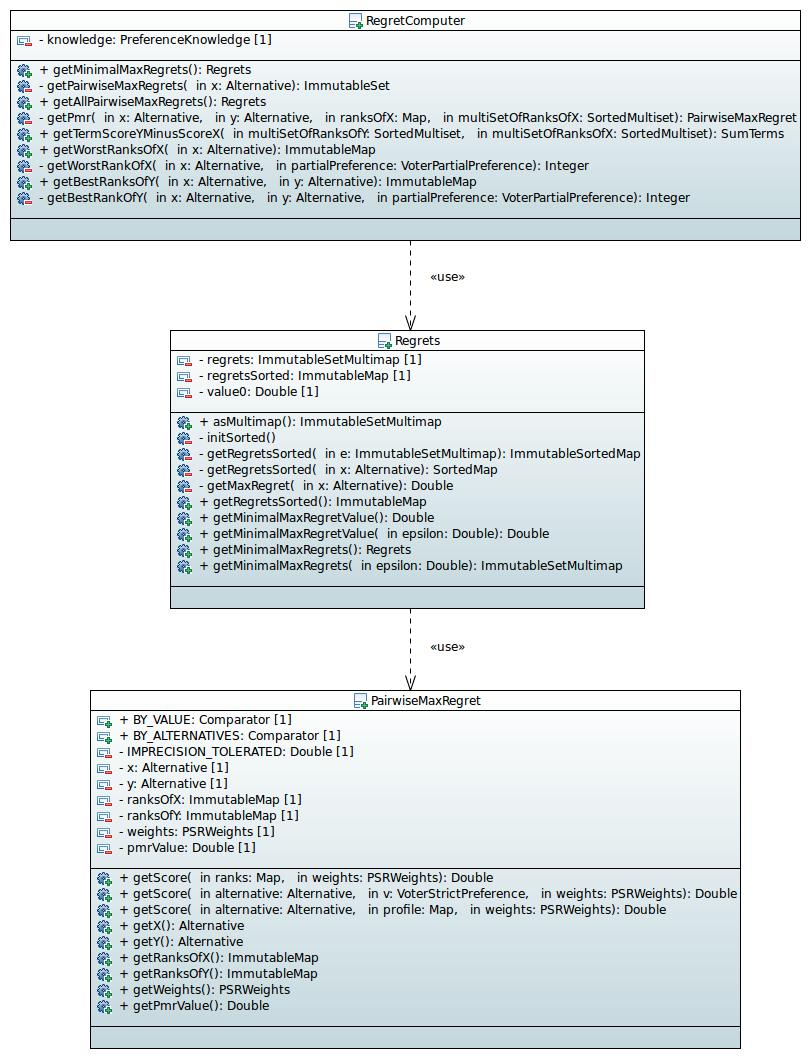
\includegraphics[width=\textwidth]{uml/regret.jpeg}
	\caption{UML class diagram of regret computation.}
	\label{uml:regret}
\end{figure}


\subsection{Strategies}

\Cref{uml:strategies} describe our design of elicitation strategies. A \textit{Strategy} is an interface that specify two methods: \textit{setKnowledge} that sets and updates the knowledge collected so far, and \textit{nextQuestion} that returns the next question to ask. Every strategy, i.e. every implementation of \textit{Strategy}, must define those two methods. We created an enumeration for the \textit{StrategyType} based on the different strategies we implemented and tested.
In particular, the ones discussed in \Cref{sec:elicit} are \textit{StrategyByMmr} that, depending on the parameters with which it is invoked, corresponds to \textit{Pessimistic}, \textit{Extended pessimistic} or \textit{Two Phases}, \textit{StrategyElitist} that corresponds to \textit{Elitist} and \textit{StrategyRandom} that corresponds to \textit{Random}.
Please see \Cref{sec:elicit} for a detailed explanation of their behaviors and performances.
From a design point of view, each strategy defines the interface methods and it makes use of a \textit{StrategyHelper} for all those functions common to each strategy. For example, to get all the pairs of alternatives whose order is already known and therefore it does not make sense to ask about; or to find the voters to whom we can still ask questions and, eventually,all those possible questions.
Finally, \textit{StrategyFactory} is an object that handles the creation of the desired strategy without disclosing to the user the strategy's creation logic.

The java package containing all those classes and also the UML diagrams can be found at \url{https://github.com/oliviercailloux/minimax}.

\begin{sidewaysfigure}
	\centering
	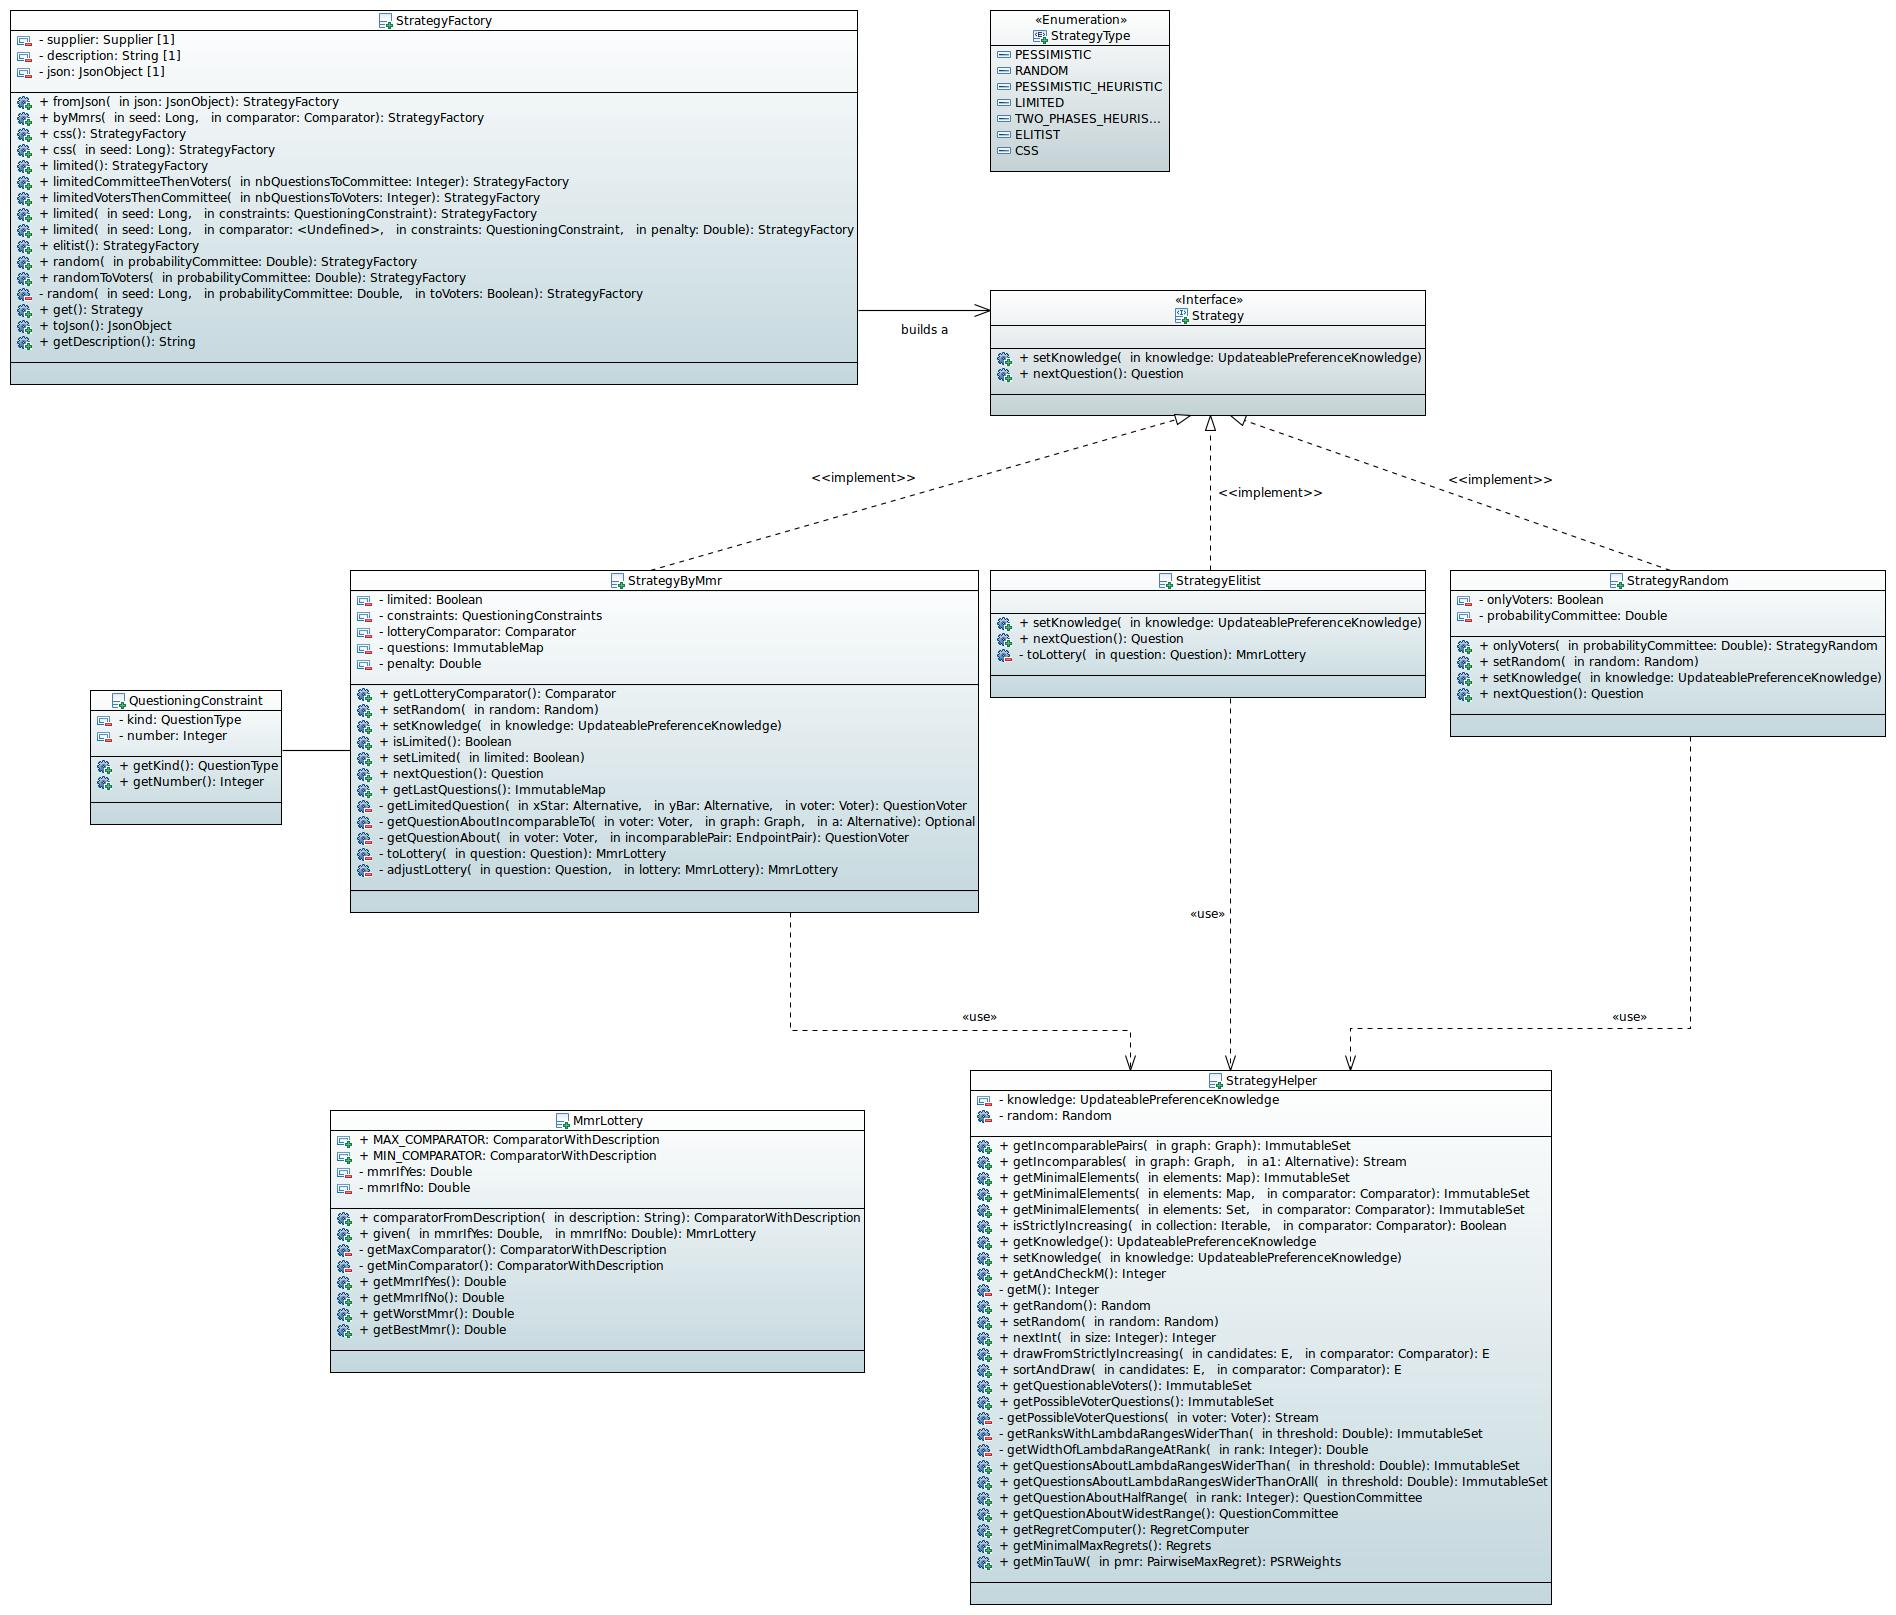
\includegraphics[width=\textwidth]{uml/strategies.jpeg}
	\caption{UML class diagram of strategies.}
	\label{uml:strategies}
\end{sidewaysfigure}
